% :wrap=soft:maxLineLen=80:

\documentclass{article}

\usepackage{type1cm}
\usepackage{texments}
\usepackage{listings}
\usepackage{graphicx}
\usepackage[colorlinks=false]{hyperref}
\usepackage[english,UKenglish]{babel}
\usestyle{default}

\newcommand{\pybool}{\emph{pybool}}
\newcommand{\hb}{\emph{hb}}
\newcommand{\pdm}{\emph{pdm}}
\newcommand{\Kr}{\emph{Kr}}
\newcommand{\cas}{\emph{cas}}
\newcommand{\svp}{\emph{svp}}
\newcommand{\X}{\emph{X}}
\newcommand{\lst}[1]{
  \begin{lstlisting}[linewidth=\textwidth, breaklines]
  #1 
  \end{lstlisting}
}
\newcommand{\hide}[1]{}
\newcommand{\todo}[1]{\textbf{[TODO: #1]}}

\usepackage{tikz}
\usetikzlibrary{snakes,arrows,shapes.geometric,decorations.pathmorphing,backgrounds,positioning,fit}
\usepgflibrary{shapes}
\pgfdeclarelayer{background}
\pgfdeclarelayer{foreground}
\pgfsetlayers{background,main,foreground}

\title{pybool: A Python package to infer Boolean networks under constraints}
\author{John Reid}

\begin{document}

\maketitle




\section{Motivation}

Consider the common scenario of a biologist who is studying a particular regulatory network. They study a set of genes that are known to play a role in the network. They have some background knowledge of particular regulatory connections from their own studies or from the literature. In addition, they have time-course perturbation data that reveal the temporal order of expression of the genes under various conditions. For example, these could be derived from loss-of-function or over-expression experiments. The biologist would like to elucidate the entire network and to this end can perform various experiments to test particular regulatory connections. These experiments are costly and time-consuming. Which connections should he focus on? This is where the \emph{pybool} package can help. By modelling candidate regulatory networks using Boolean logic, \emph{pybool} evaluates which networks are consistent with the perturbation data and the known regulatory connections. The biologist can then examine the consistent networks to determine which unknown regulatory connections are most promising for further experimentation.



\subsection{Boolean networks}
Kaufman~\cite{Kauffman1969} and Thomas~\cite{Thomas1973} proposed \emph{Boolean networks} in 1969 and 1973 respectively. Davidson et al.~\cite{Davidson2002} used them to model the development of the sea urchin embryo. Giacomantonio and Goodhill used them to model mammalian cortical area development~\cite{Giacomantonio2010}. Li et al.~\cite{Li2004} analysed the robustness of the yeast cell-cycle regulatory network using Boolean networks with threshold functions. Shmulevich et al.~\cite{Shmulevich2002} extended Boolean networks to incorporate probabilistically determined regulation functions. Karlebach and Shamir have reviewed Boolean networks as models of gene regulatory networks~\cite{Karlebach2008}. Akutsu et al.~\cite{Akutsu1999} and L\"{a}hdesm\"{a}ki et al.~\cite{Lahdesmaki2003} provide algorithms for the \emph{consistency problem}, that is finding those networks that agree with observations.

In its most general form, a Boolean network, \(G(V, F)\), consists of a set of nodes with initial values, \(V = \{X_1^0,\dots,X_N^0\}\), and a set of Boolean functions, \(F = \{f_1,\dots,f_N\}, f_i : \{0, 1\}^N \mapsto \{0, 1\}\). When modelling gene regulatory networks, \(X_i^t \in \{0, 1\}\) represents the expression state of gene \(i\) at time \(t\) where \(0 \le t \le T\). The dynamics of the network are defined by \(F\), \(X_i^t = f_i(X_i^{t-1})\).



\section{Methods}
Our Boolean network model follows that of Nakajima et al.~\cite{Nakajima2010} which is in turn based on that of Li et al.~\cite{Li2004}. In these models, the functions, \(f_i\), are restricted to be of a particular threshold type
\begin{equation}
X_i^{t+1} = f_i(\mathbf{X}^t) = \left\{ \begin{array}{cl}
  1 & \textrm{if $\sum_j J_{ij} X_j^t > 0$} \\
  0 & \textrm{if $\sum_j J_{ij} X_j^t < 0$} \\
  \theta_i & \textrm{if $\sum_j J_{ij} X_j^t = 0$}
\end{array} \right.
\label{eq:recurrence}
\end{equation}
As above, $X_i^t$ is the expression state of gene $i$ at time point $t$ and can be on (1) or off (0). $J_{ij}$ represents the regulatory effect of gene $j$ on gene $i$. $J_{ij} > 0$, $J_{ij} < 0$ and $J_{ij} = 0$  imply activation, repression and the absence of regulation respectively. $\theta_i \in \{0,1\}$ is the constitutive expression state of gene $i$, that is it determines whether the gene is off or on in the absence of activation and repression. A network is fully specified by \(F = F(J, \theta)\) and a set of initial conditions, $V = \{X_i^0\}$. The recurrence relation (\ref{eq:recurrence}) allows us to run the network forward through time and achieve a \emph{realisation} of the network, $\{X_i^t\ : 0 \le t \le T\}$.

It is not possible to model all regulatory relationships as threshold functions. The simplest relationship that cannot be modelled as a threshold is an exclusive-or relationship where a regulated gene is on when exactly one of its two regulating genes is on. Nevertheless threshold functions are able to model most of the typical regulatory relationships seen in recently characterised genetic networks. On the other hand, this lack of flexibility is not necessarily a drawback. It may well be that the regulatory relationships that cannot be modelled by threshold functions are not common in nature. For example they may not be implemented easily on a molecular level or perhaps they exhibit some property such as instability that makes them evolutionarily unattractive. In any case, focussing our attention on threshold functions does not seem overly restrictive and also brings some beneficial side-effects. In general form, Boolean functions are most economically represented by a truth table that has \(2^N\) entries where \(N\) is the number of input genes. These large tables make interpretation of inferred functions difficult. For similar reasons of size, integrating prior knowledge of regulatory relationships is not easy. For example, we may know that gene A has an activatory effect on gene B. In the threshold function formalism this is easily encoded. It is not obvious there is an intuitive way to do this with a generalised truth table.




\subsection{The consistency problem}
Returning to the problem at hand, the biologist is interested in those networks that agree with their understanding of which regulatory connections are possible and that also lead to realisations that agree with their time-course perturbation data. This is known as the consistency problem (L\"{a}hdesm\"{a}ki et al.~\cite{Lahdesmaki2003}). To use \pybool\ to solve this problem, the biologist defines a set of \emph{restrictions} and a set of \emph{conditions}. The restrictions limit the space of networks by constraining the possible regulatory connections. Each condition is associated with a perturbation data set and has \emph{constraints} associated with it. Each constraint represents the observed temporal order of gene expression in the data set. \pybool\ examines each network in the restricted space and tests if its realisations for each condition satisfy the condition's constraints. Those that do satisfy all the conditions' constraints are the \emph{consistent} networks.

Restrictions take the form of sets of valid values for the parameters that define the network,  $J$, $\theta$ and $\{X_i^0\}$. These reflect which parameters the biologist is confident about. The restrictions limit the size of the network space that \pybool\ searches. The search space grows exponentially with the permitted regulatory connections so it is in the biologist's interests to restrict the search space as much as possible. Connections can be constrained to be absent, activatory, repressive or a combination of the above.

A condition and its associated constraints model the information a biologist has from a time-course pertubation experiment. For example, when a particular gene is over-expressed, time-course microarrays may reveal the temporal order of gene expression. When searching the network space for consistent networks, \pybool\ will override the recurrence relation (\ref{eq:recurrence}) to reflect the perturbations made in the experiment and generate realisations that can be checked against the condition's constraints. A condition is not limited to one perturbation, it is possible to define a condition that models the combination of multiple knock-downs or over-expressions.

The biologist can also define genes as \emph{external inputs}. External inputs represent knowledge the biologist may have regarding external signals coming into the regulatory network. They are encoded as functions that tell \pybool\ to fix the values of the external input gene at each time point.





\subsection{Comparison to existing software}

A brief round-up of other software for Boolean networks:
\begin{itemize}
\item BoolNet in R by M\"ussel et al.~\cite{Muessel2010}. Solves the consistency problem with the REVEAL algorithm and has a best-fit extension implementation. Cannot integrate expert knowledge into threshold functions explicitly. Artistic License 2.0.
\item Matlab Random Boolean Network Toolbox by Schwarzer~\url{http://www.teuscher.ch/rbntoolbox/index.htm}. Finds attractors. Does not seem to solve the consistency problem.
\item Matlab PBN toolbox by Shmulevich et al.~\cite{Shmulevich2002}. Infers network from data. No documentation outside of MatLab so hard to determine if handles threshold functions. Uses MatLab.
\item NetBuilder~\cite{Brown2002} and NetBuilder'~\cite{Wegner2007} by Schilstra et al. \url{http://strc.herts.ac.uk/bio/maria/NetBuilder}. Does not appear to infer networks from data, is more of a simulation tool.
\item DDLab by Andy Wuensche~\url{http://www.ddlab.com/}. Needs license for academic and other use except for personal. Huge manual mainly focussed on attractors.
\item BooleanNet by Albert et al.~\cite{Albert2008}. Appears to be a simulator of networks rather than an inferrer of networks. MIT Open Source License.
\item CellNetAnalyzer by Klamt et al.~\cite{Klamt2007}. This runs in Matlab. Another simulator rathan than an inferrer. Free academic license.
\end{itemize}





\section{Running \pybool}

We illustrate how \pybool\ works using an example from a paper by Nakajima et al.~\cite{Nakajima2010}. They are interested in the regulatory network that controls neurogenesis in Drosophila. Their system consists of six genes, \hb, \Kr, \pdm, \cas, \svp\ and \X. They have loss-of-function and over-expression time-course data for \hb, \Kr, \pdm\ and \cas. \svp\ and \X\ are regarded as external inputs to the system.

Once \pybool\ has been installed (see Section~\ref{sec:installation}) it can be run via its command-line interface
\pygment{bash}{pybool_run_constraints.py --plot 5 pybool.examples.tutorial}
Here we have run the \verb!pybool_run_constraints.py! Python script and passed an argument \verb!pybool.examples.tutorial!. The argument is the name of a Python module that contains all information about the conditions and constraints. \verb!--plot 5! is an option that asks \pybool\ to plot a graph of the first five of the consistent networks.

\begin{figure}[!tpb]
\center

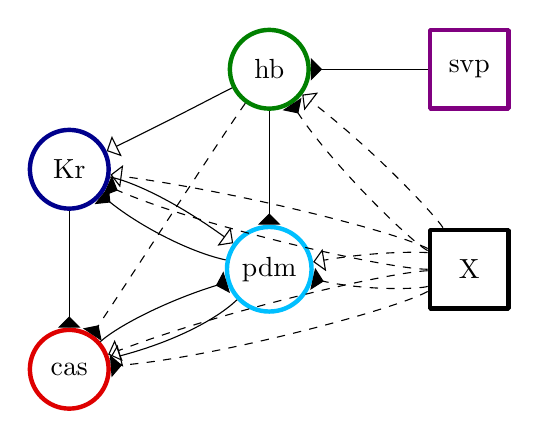
\begin{tikzpicture}[>=latex,line join=bevel,]
%%
\begin{scope}[ultra thick,minimum size=1cm]
  \definecolor{strokecolor}{rgb}{0.0,0.5,0.0};
  \node (1) at (84bp,120bp) [draw=strokecolor,circle] {hb};
  \definecolor{strokecolor}{rgb}{0.5,0.0,0.5};
  \node (0) at (156bp,120bp) [draw=strokecolor,rectangle] {svp};
  \definecolor{strokecolor}{rgb}{0.0,0.75,1.0};
  \node (3) at (84bp,48bp) [draw=strokecolor,circle] {pdm};
  \definecolor{strokecolor}{rgb}{0.0,0.0,0.55};
  \node (2) at (12bp,84bp) [draw=strokecolor,circle] {Kr};
  \definecolor{strokecolor}{rgb}{0.0,0.0,0.0};
  \node (5) at (156bp,48bp) [draw=strokecolor,rectangle] {X};
  \definecolor{strokecolor}{rgb}{0.87,0.0,0.0};
  \node (4) at (12bp,12bp) [draw=strokecolor,circle] {cas};
\end{scope}
  \draw [->,-open triangle 90] (2) ..controls (33bp,80bp) and (48bp,74bp)  .. (3);
  \draw [->,-triangle 90 reversed,dashed] (5) ..controls (128bp,33bp) and (63bp,16bp)  .. (4);
  \draw [->,-open triangle 90,dashed] (5) ..controls (128bp,47bp) and (70bp,34bp)  .. (4);
  \draw [->,-triangle 90 reversed] (1) ..controls (84bp,99bp) and (84bp,84bp)  .. (3);
  \draw [->,-triangle 90 reversed,dashed] (1) ..controls (65bp,93bp) and (38bp,51bp)  .. (4);
  \draw [->,-triangle 90 reversed,dashed] (5) ..controls (139bp,41bp) and (120bp,40bp)  .. (3);
  \draw [->,-open triangle 90,dashed] (5) ..controls (141bp,54bp) and (126bp,55bp)  .. (3);
  \draw [->,-triangle 90 reversed,dashed] (5) ..controls (127bp,48bp) and (60bp,63bp)  .. (2);
  \draw [->,-open triangle 90,dashed] (5) ..controls (128bp,62bp) and (72bp,76bp)  .. (2);
  \draw [->,-open triangle 90] (3) ..controls (65bp,30bp) and (50bp,22bp)  .. (4);
  \draw [->,-triangle 90 reversed] (3) ..controls (56bp,54bp) and (38bp,63bp)  .. (2);
  \draw [->,-triangle 90 reversed] (0) ..controls (134bp,120bp) and (116bp,120bp)  .. (1);
  \draw [->,-triangle 90 reversed,dashed] (5) ..controls (136bp,57bp) and (107bp,85bp)  .. (1);
  \draw [->,-open triangle 90,dashed] (5) ..controls (144bp,67bp) and (123bp,90bp)  .. (1);
  \draw [->,-triangle 90 reversed] (4) ..controls (30bp,28bp) and (48bp,37bp)  .. (3);
  \draw [->,-open triangle 90] (1) ..controls (64bp,110bp) and (49bp,102bp)  .. (2);
  \draw [->,-triangle 90 reversed] (2) ..controls (12bp,61bp) and (12bp,45bp)  .. (4);
%
\end{tikzpicture}


\caption{The possible networks. Dashed edges represent regulatory connections that may not exist. Square nodes are external inputs. Open triangle arrow tips represent activation and filled reversed triangle arrow tips represent repression.}
\label{fig:restrictions}
\end{figure}




Let's have a look at some of the output \pybool\ produces. To start with \pybool\ outputs information about the restrictions.
\lstdefinestyle{output}{basicstyle=\small,linewidth=\textwidth, breaklines}
\begin{lstlisting}[style=output]
The possible regulatory relationships are:
[[        svp     hb     Kr    pdm    cas     X   ]
 [ svp     0      0      0      0      0      0   ]
 [  hb     -      0      0      0      0    -/0/+ ]
 [  Kr     0      +      0      -      0    -/0/+ ]
 [ pdm     0      -      +      0      -    -/0/+ ]
 [ cas     0     -/0     -      +      0    -/0/+ ]
 [  X      0      0      0      0      0      0   ]]
The possible constitutive expression levels are:
    svp : (0,)
     hb : (0, 1)
     Kr : (0, 1)
    pdm : (0, 1)
    cas : (0, 1)
      X : (0,)
    svp is an external input with possible input parameters: None
      X is an external input with possible input parameters: 1,2,3,4,5,6,7,8,9,10,11
\end{lstlisting}
These define the possible $J$s, $\theta$s and external input parameters for the networks we will test. In the $J$ matrix, the columns are the regulators and the rows are the regulated genes. For example we see that \svp\ and \X\ cannot be regulated but can regulate other genes. \pybool\ will also output a graph showing the possible $J$s (see Figure~\ref{fig:restrictions}).

We see some information about what \pybool\ will do. It tells us how many different networks it will test against which conditions.
\begin{lstlisting}[style=output]
The conditions to test are: wt, hb-, Kr-, pdm-, cas-, hb++, Kr++, pdm++, cas++
Will generate 28512 different networks.
\end{lstlisting}

When it has completed testing the networks, we see a summary of the results
\begin{lstlisting}[style=output]
Evaluated 28512 networks in 5.4 seconds. 5273.5/sec
Total mismatches = 99192
Found 27368 networks which match the default condition "wt" (161 distinct Js).
Found 149 consistent networks which match all conditions (17 distinct Js).
Condition broken count:      wt = 26873
Condition broken count:     hb- = 995
Condition broken count:     Kr- = 243
Condition broken count:    pdm- = 252
Condition broken count:    cas- = 0
Condition broken count:    hb++ = 0
Condition broken count:    Kr++ = 0
Condition broken count:   pdm++ = 0
Condition broken count:   cas++ = 0
\end{lstlisting}
Here only 149 out of the 28,512 possible networks satisfied the constraints in all conditions. Each one of the 149 is a different combination of $J$ and $\theta$. In all there were only 17 unique $J$s in the 149. The remaining variation in the consistent networks comes from the $\theta$s. We are also shown counts of the number of networks which did not satisfy each condition. Note that the conditions are tested in a particular order. Once one condition has failed, \pybool\ does not evaluate the other conditions so these counts are skewed towards the earlier conditions.

Now we see a summary of the 149 consistent networks
\begin{lstlisting}[style=output]
The consistent regulatory relationships in the networks are:
[[        svp     hb     Kr    pdm    cas     X   ]
 [ svp     0      0      0      0      0      0   ]
 [  hb     -      0      0      0      0    -/0/+ ]
 [  Kr     0      +      0      -      0      +   ]
 [ pdm     0      -      +      0      -    -/0/+ ]
 [ cas     0     -/0     -      +      0      -   ]
 [  X      0      0      0      0      0      0   ]]
Valid constitutive expression levels for     svp are 0
Valid constitutive expression levels for      hb are 0
Valid constitutive expression levels for      Kr are 0
Valid constitutive expression levels for     pdm are 0,1
Valid constitutive expression levels for     cas are 1
Valid constitutive expression levels for       X are 0
Valid input parameters for the external input of     svp are: None
Valid input parameters for the external input of       X are: 1,2,3,4,5,6,7,8,9
\end{lstlisting}
We can see that in the consistent networks, \X\ always activates \Kr\ and represses \cas. Only some of the tested constitutive expression levels are possible. Most of the possible input parameters that control the timing of \X\ are consistent. The possible $J$s are summarised in Figure~\ref{fig:consistent}.

Because we included the command-line option \verb!--plot 5! we will have 5 networks and their realisations plotted. See Figure~\ref{fig:network} for an example.

\begin{figure}[!tpb]
\center

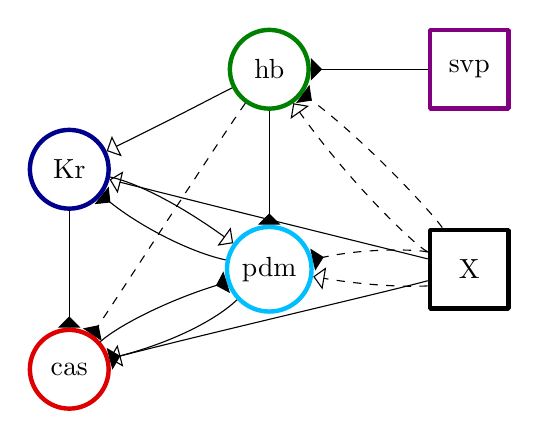
\begin{tikzpicture}[>=latex,line join=bevel,]
%%
\begin{scope}[ultra thick,minimum size=1cm]
  \definecolor{strokecolor}{rgb}{0.0,0.5,0.0};
  \node (1) at (84bp,120bp) [draw=strokecolor,circle] {hb};
  \definecolor{strokecolor}{rgb}{0.5,0.0,0.5};
  \node (0) at (156bp,120bp) [draw=strokecolor,rectangle] {svp};
  \definecolor{strokecolor}{rgb}{0.0,0.75,1.0};
  \node (3) at (84bp,48bp) [draw=strokecolor,circle] {pdm};
  \definecolor{strokecolor}{rgb}{0.0,0.0,0.55};
  \node (2) at (12bp,84bp) [draw=strokecolor,circle] {Kr};
  \definecolor{strokecolor}{rgb}{0.0,0.0,0.0};
  \node (5) at (156bp,48bp) [draw=strokecolor,rectangle] {X};
  \definecolor{strokecolor}{rgb}{0.87,0.0,0.0};
  \node (4) at (12bp,12bp) [draw=strokecolor,circle] {cas};
\end{scope}
  \draw [->,-open triangle 90] (2) ..controls (33bp,80bp) and (48bp,74bp)  .. (3);
  \draw [->,-triangle 90 reversed] (5) ..controls (127bp,40bp) and (62bp,25bp)  .. (4);
  \draw [->,-triangle 90 reversed] (1) ..controls (84bp,99bp) and (84bp,84bp)  .. (3);
  \draw [->,-triangle 90 reversed,dashed] (1) ..controls (65bp,93bp) and (38bp,51bp)  .. (4);
  \draw [->,-open triangle 90,dashed] (5) ..controls (141bp,42bp) and (126bp,41bp)  .. (3);
  \draw [->,-triangle 90 reversed,dashed] (5) ..controls (139bp,55bp) and (120bp,56bp)  .. (3);
  \draw [->,-open triangle 90] (5) ..controls (128bp,55bp) and (71bp,69bp)  .. (2);
  \draw [->,-open triangle 90] (3) ..controls (65bp,30bp) and (50bp,22bp)  .. (4);
  \draw [->,-triangle 90 reversed] (3) ..controls (56bp,54bp) and (38bp,63bp)  .. (2);
  \draw [->,-triangle 90 reversed] (0) ..controls (134bp,120bp) and (116bp,120bp)  .. (1);
  \draw [->,-open triangle 90,dashed] (5) ..controls (137bp,56bp) and (113bp,79bp)  .. (1);
  \draw [->,-triangle 90 reversed,dashed] (5) ..controls (143bp,68bp) and (118bp,95bp)  .. (1);
  \draw [->,-triangle 90 reversed] (4) ..controls (30bp,28bp) and (48bp,37bp)  .. (3);
  \draw [->,-open triangle 90] (1) ..controls (64bp,110bp) and (49bp,102bp)  .. (2);
  \draw [->,-triangle 90 reversed] (2) ..controls (12bp,61bp) and (12bp,45bp)  .. (4);
%
\end{tikzpicture}


\caption{The consistent networks that satisfy the constraints in the Nakajima et al. example.}
\label{fig:consistent}
\end{figure}


\begin{figure}[!tpb]
\center

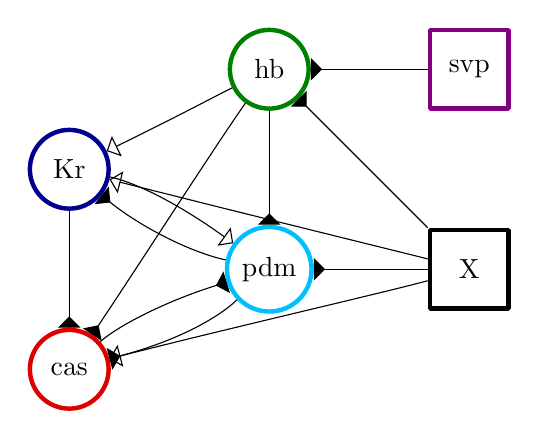
\begin{tikzpicture}[>=latex,line join=bevel,]
%%
\begin{scope}[ultra thick,minimum size=1cm]
  \definecolor{strokecolor}{rgb}{0.0,0.5,0.0};
  \node (1) at (84bp,120bp) [draw=strokecolor,circle] {hb};
  \definecolor{strokecolor}{rgb}{0.5,0.0,0.5};
  \node (0) at (156bp,120bp) [draw=strokecolor,rectangle] {svp};
  \definecolor{strokecolor}{rgb}{0.0,0.75,1.0};
  \node (3) at (84bp,48bp) [draw=strokecolor,circle] {pdm};
  \definecolor{strokecolor}{rgb}{0.0,0.0,0.55};
  \node (2) at (12bp,84bp) [draw=strokecolor,circle] {Kr};
  \definecolor{strokecolor}{rgb}{0.0,0.0,0.0};
  \node (5) at (156bp,48bp) [draw=strokecolor,rectangle] {X};
  \definecolor{strokecolor}{rgb}{0.87,0.0,0.0};
  \node (4) at (12bp,12bp) [draw=strokecolor,circle] {cas};
\end{scope}
  \draw [->,-open triangle 90] (2) ..controls (33bp,80bp) and (48bp,74bp)  .. (3);
  \draw [->,-triangle 90 reversed] (5) ..controls (127bp,40bp) and (62bp,25bp)  .. (4);
  \draw [->,-triangle 90 reversed] (1) ..controls (84bp,99bp) and (84bp,84bp)  .. (3);
  \draw [->,-triangle 90 reversed] (1) ..controls (65bp,93bp) and (38bp,51bp)  .. (4);
  \draw [->,-triangle 90 reversed] (5) ..controls (140bp,48bp) and (122bp,48bp)  .. (3);
  \draw [->,-open triangle 90] (5) ..controls (128bp,55bp) and (71bp,69bp)  .. (2);
  \draw [->,-open triangle 90] (3) ..controls (65bp,30bp) and (50bp,22bp)  .. (4);
  \draw [->,-triangle 90 reversed] (3) ..controls (56bp,54bp) and (38bp,63bp)  .. (2);
  \draw [->,-triangle 90 reversed] (0) ..controls (134bp,120bp) and (116bp,120bp)  .. (1);
  \draw [->,-triangle 90 reversed] (5) ..controls (138bp,66bp) and (113bp,91bp)  .. (1);
  \draw [->,-triangle 90 reversed] (4) ..controls (30bp,28bp) and (48bp,37bp)  .. (3);
  \draw [->,-open triangle 90] (1) ..controls (64bp,110bp) and (49bp,102bp)  .. (2);
  \draw [->,-triangle 90 reversed] (2) ..controls (12bp,61bp) and (12bp,45bp)  .. (4);
%
\end{tikzpicture}


\vspace{.5cm}
%\includegraphics[width=.95\textwidth]{Figures/net-001}
\includegraphics[width=.95\textwidth]{Figures/net-realisations-001-bbox}
\caption{\emph{Top}: One of the consistent networks that satisfies the constraints in the Nakajima et al. example. \emph{Below}: Graphical representations of the realisations for each of the conditions. Time is represented on the y-axis and the genes are colour-coded as in the network above.}
\label{fig:network}
\end{figure}



\subsection{Running in parallel}

Checking which networks are consistent is trivially parallelisable. \pybool\ uses the simple yet powerful IPython package for parallelisation (see \url{http://ipython.scipy.org/doc/stable/html/parallel/index.html}). To run \pybool\ in parallel mode is as easy as starting an \verb!ipcluster! with the desired number of engines
\pygment{bash}{ipcluster local -n 2}
and then running \pybool\ with the \verb!-p! command-line option
\pygment{bash}{pybool_run_constraints.py -p pybool.examples.tutorial}
The task will then be distributed over all the engines in the \verb!ipcluster!.



\subsection{Other options}

\begin{itemize}
\item \verb!--black-and-white! will generate black and white network diagrams.
\item \verb!-m=N! will limit the number of networks examined to \verb!N!.
\item \verb!--use-LaTeX! will generate network diagrams in LaTeX using the tikz package. This option is provided for publication quality figures. However the standard network diagrams are of a reasonable quality in any case.
\item \verb!-F=<format>! will add the format to the list of formats that the network diagrams are generated in. Any format supported by GraphViz and matplotlib is permissible, for example eps, or pdf. png is the default format. 
\item \verb!-h! will display all the possible options.
\end{itemize}



\section{Configuration}

Now we have seen how to run \pybool, we can examine how to configure the conditions and the constraints. Let's look at the Python code in the module \verb!pybool.examples.tutorial!. The \pybool\ code interfaces with the module via the \verb!MetaData! class
\begin{pygmented}{python}
class MetaData(BaseMetaData):
    """
    Meta-data for drosophila neurogenesis regulatory 
    networks in Nakajima paper.
    """
\end{pygmented}
\pybool\ will instantiate an instance of this class and query its attributes for the conditions and constraints. First of all we set up the basic info in the class's constructor
\begin{pygmented}{python}
    def __init__(self):
        "Construct."
        
        BaseMetaData.__init__(self)

        self.genes = (
            'svp',  # 0
            'hb',   # 1
            'Kr',   # 2
            'pdm',  # 3
            'cas',  # 4
            'X',    # 5
        )
        "The gene names."

        self.G = len(self.genes)
        "The number of genes."

        self.T = 12
        "The number of time steps to realise."
\end{pygmented}
Next we define the conditions and which genes are forced on or off in each
\begin{pygmented}{python}
        self.conditions = [
            'wt',
            'hb-',
            'Kr-',
            'pdm-',
            'cas-',
            'hb++',
            'Kr++',
            'pdm++',
            'cas++',
        ]
        "Conditions."

        self.condition_inputs = {
            'wt'    : { },
            'hb-'   : {  HB : gene_off },
            'Kr-'   : {  KR : gene_off },
            'pdm-'  : { PDM : gene_off },
            'cas-'  : { CAS : gene_off },
            'hb++'  : {  HB : gene_on },
            'Kr++'  : {  KR : gene_on },
            'pdm++' : { PDM : gene_on },
            'cas++' : { CAS : gene_on },
        }
        """
        Condition input functions that map genes 
        to fixed expression states (up or down).
        """

        self.default_condition = 'wt'
        "The condition to use if none specified."
\end{pygmented}
We define the external inputs, each one is defined as a function that takes a parameter
\begin{pygmented}{python}
        self.external_inputs = {
            # svp is on at time=1
            SVP : svp_external_input,
            
            # X is activated at time < parameter
              X : X_external_input,
        }
        """
        Default external inputs into the network (can be over-ridden
        when generating a realisation for a particular condition).
        """
\end{pygmented}
The algorithm needs to be provided with initial expression states for each gene
\begin{pygmented}{python}
        # All initial states are 0 except for HB and X
        self.initial_states = N.zeros((self.G,), dtype=int)
        "Initial expression states."
        self.initial_states[HB] = 1
        self.initial_states[X] = 1
\end{pygmented}
In the following code we define which regulatory connections are possible
\begin{pygmented}{python}
        # set up the possible regulatory connections
        self.possible_Js = N.empty((self.G, self.G), dtype=object)
        "Possible values of J."        
        unconstrained = (-5, 0, 1)
        represses_or_none = (-5, 0)
        activates = (1,)
        represses = (-5,)
        no_regulation = (0,)
        
        # initialise all connections to unconstrained
        for g1 in xrange(self.G):
            for g2 in xrange(self.G):
                self.possible_Js[g1, g2] = no_regulation
        
        # X can regulate any of HB, KR, PDM and CAS
        self.possible_Js[  X, HB] = unconstrained
        self.possible_Js[  X, KR] = unconstrained
        self.possible_Js[  X,PDM] = unconstrained
        self.possible_Js[  X,CAS] = unconstrained
        
        # from Figure 1 in Nakajima paper
        self.possible_Js[SVP, HB] = represses
        self.possible_Js[ HB, KR] = activates
        self.possible_Js[ HB,PDM] = represses
        self.possible_Js[ HB,CAS] = represses_or_none
        self.possible_Js[ KR,PDM] = activates
        self.possible_Js[ KR,CAS] = represses
        self.possible_Js[PDM, KR] = represses
        self.possible_Js[PDM,CAS] = activates
        self.possible_Js[CAS,PDM] = represses
\end{pygmented}
We set the possible constitutive expression levels. These are irrelevant for the external input genes, \svp\ and \X\ so we set them to off.
\begin{pygmented}{python}
        # possible constitutive expression levels
        self.possible_thetas = N.empty((self.G), dtype=object)
        "Possible values of theta."
        unconstrained = (0, 1)
        for g in xrange(self.G):
            # thetas for external inputs are irrelevant
            if g in self.external_inputs:
                self.possible_thetas[g] = (0,)
            else:
                self.possible_thetas[g] = unconstrained
\end{pygmented}
However the external inputs are parameterised and we have to define the possible parameter sets.
\begin{pygmented}{python}
        # set up all possible input parameters.
        self.possible_input_params = [(None,)] * self.G
        "The possible input parameters."
        self.possible_input_params[X] = N.arange(1, self.T)
\end{pygmented}
We provide some details that allow \pybool\ to create graphics of the networks. We define a colour for each gene and a fixed position for when the network is drawn.
\begin{pygmented}{python}
        self.colours = N.array((
            M.colors.colorConverter.to_rgb('purple'),
            M.colors.colorConverter.to_rgb('green'),
            M.colors.colorConverter.to_rgb('darkblue'),
            M.colors.colorConverter.to_rgb('deepskyblue'),
            M.colors.colorConverter.to_rgb('#DD0000'),
            M.colors.colorConverter.to_rgb('black'),
        ))
        "Colours to use when plotting realisations, etc..."

        self.graph_positions = {
            SVP : ( 2, 3),
             HB : ( 0, 3),
             KR : (-2, 2),
            PDM : ( 0, 1),
            CAS : (-2, 0),
              X : ( 2, 1),
        }
        "Fixed positions of the genes in a graph."
\end{pygmented}
Finally we call a base class method that makes sure we limit the set of possible networks to those that are relevant. For example this enforces that external inputs can only have one constitutive expression level.
\begin{pygmented}{python}
        # make sure we don't allow regulation of inputs, etc..
        self._tighten_constraints_on_inputs()
\end{pygmented}




\section{Conclusions}

Due to current levels of ignorance about most regulatory networks, the simplest models can often be the most practical for modelling. Thresholded Boolean network functions fit into this category. When combined with qualitative constraints on the order of gene expression they offer an attractive method of investigating regulatory networks.

Python is a well regarded and easy to use language. Our parallelisable C++ implementation can efficiently analyse tens of thousands of networks per second.

\pybool\ offers a range of graphical outputs to make interpretation of the results easier. Several different image formats are supported.




\section{License}

\pybool\ is free for academic use. For commercial licenses please contact the author

\begin{verbatim}
  John Reid,
  MRC Biostatistics Unit,
  Institute of Public Health,
  University Forvie Site,
  Robinson Way,
  Cambridge.
  CB2 0SR.
\end{verbatim}



\section{Appendix: Installation}

\label{sec:installation}

The \verb!README! file that comes with the pybool source download covers the installation instructions. See~\url{http://sysbio.mrc-bsu.cam.ac.uk/johns/pybool/}.





%\bibliographystyle {natbib}
%\renewcommand{\bibname}{Bibliography} % changes the header; default: Bibliography
 %\nocite{*}
\bibliography{bibliography} % adjust this to fit your BibTex file
\bibliographystyle{plain}

\end{document}

